\chapter{Introducción}
\label{ch:intro}

\section{Sección Uno}
\subsection{Apartado Uno}
\label{sec:apartado1}

\noindent Texto del \autoref{sec:apartado1}. \lipsum[1]

\begin{itemize}
    \item Item 1
    \item Item 2
    \item Item 3
    \item Item 4
\end{itemize}

Más texto del \autoref{sec:apartado1} antes del \autoref{sec:sección2}. \lipsum[2]

\section{Sección Dos}
\label{sec:sección2}

\begin{enumerate}
    \item Item 1
    \item Item 2
    \item Item 3
\end{enumerate}

\section{Sección Tres}

\noindent Bla, bla en la \autoref{fig:intro}, bla... \lipsum[3]

\begin{figure}[htb]
   \centering
   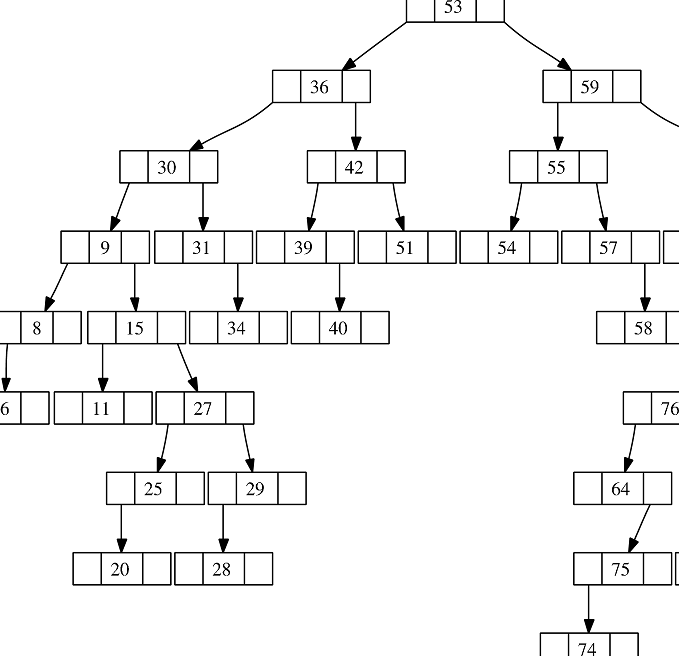
\includegraphics[width=0.8\linewidth]{images/figura_1}
   \caption{Ejemplo de figura.}
   \label{fig:intro}
\end{figure}

\lipsum[4]

\section{Sección Cuatro}

\noindent \lipsum[5-6]